% Assignment 4 research report. Build from assignment4/report/ with:
%   tectonic -X compile main.tex
% Tables and figures are read from ../analysis (generated by analysis/analyze.py).
\documentclass[11pt,a4paper]{article}

\usepackage[T1]{fontenc}
\usepackage{lmodern}
\usepackage{microtype}
\usepackage[margin=2.4cm]{geometry}
\usepackage{amsmath}
\usepackage{booktabs}
\usepackage{array}
\usepackage{graphicx}
\usepackage{xcolor}
\usepackage{listings}
\usepackage[font=small,labelfont=bf]{caption}
\usepackage{enumitem}
\usepackage[hidelinks]{hyperref}
\usepackage{url}
\usepackage[section]{placeins} % floats stay within their section

\graphicspath{{../analysis/figures/}}
\newcommand{\tabledir}{../analysis/tables}
\newcommand{\repourl}{\url{https://github.com/Xami650/Individual-Assignments-Big-Data-ULPGC}}
\newcommand{\session}{\texttt{20261120-031850}}

\lstset{
  basicstyle=\ttfamily\footnotesize,
  columns=fullflexible,
  keepspaces=true,
  frame=single,
  framesep=3pt,
  rulecolor=\color{black!30},
  aboveskip=4pt,
  belowskip=2pt,
  showstringspaces=false,
}

\setlist{itemsep=2pt,topsep=4pt}
\setlength{\emergencystretch}{3em}

\title{\textbf{Assignment 4: Distributed Matrix Multiplication with Hazelcast}\\[4pt]
\large Scaling a Row-Band Decomposition over 1 to 10 Workers,\\
with Setup, Transfer and Computation Separated\\[2pt]
\normalsize (local execution: one machine, $w$ member processes, loopback TCP)}
\author{Máximo Prosperi Reynoso\\[2pt]
\small BIG DATA, GCID, ULPGC\\
\small Individual Assignment 4, 2026--2027\\[2pt]
\small \repourl}
\date{November 2026}

\begin{document}
\maketitle

\begin{abstract}
\noindent
This study distributes the validated i-k-j matrix multiplication of the earlier
assignments over a Hazelcast cluster of $w=1$ to 10 member processes, with one
band of rows of $A$, a copy of $B$ and the task that computes the band placed
explicitly on each member, and compares it with the sequential and the
shared-memory parallel versions on the same ten cores. All processes ran on one
Apple M4 laptop over loopback TCP (local execution), so the results measure the
framework and separate processes, not a network. The product is bitwise
identical to the sequential kernel for every configuration, and the bytes moved
are the predicted $(w+2)\,8n^2$ within 0.05\%. The distributed version is never
faster than threads on the same bands: its best speedup over the sequential
kernel is 0.86 at $n=256$, 1.4 to 1.5 for $n=512$ to 2048 and 2.5 at $n=4096$,
against 3.6 to 4.9 for the threads, and distributing the same bands costs 1.03
to 7 times their time. Communication (serialization, transfers and
deserialization at 2 to 11~GB/s) dominates only for $n\le512$; from $n=1024$ on
the main cost is that $w$ processes with $w$ private copies of $B$ compute more
slowly than threads sharing one (up to 2.6 times the cycles per multiply-add),
which also makes one member of ten threads faster than ten members of one. In
weak scaling dist stays 1.7 to 2.3 times slower than the threads, whose own
efficiency also falls, to 0.30 at eight workers on one chip. Forming a cluster takes
about 10~s, and its memory grows by about 0.9~GiB per member at $n=4096$. The
same kernel was also found to run at two speeds with identical instructions,
which depend on memory placement rather than on the matrix size.
\end{abstract}

% ===========================================================================
\section{Introduction and objective}

Assignment~3 split the rows of the validated i-k-j kernel among the threads of
one Java process. The threads shared one copy of the matrices, so no data had
to be moved, and ten threads made a multiplication about three to four times
faster on the ten cores of an Apple M4~\cite{a3report}. A distributed
framework removes the shared memory: each worker is a separate process with
its own heap, possibly on another machine. The data must be split, sent to the
workers and the results collected, and the framework itself has a cost. This
study keeps the kernel and the row split of Assignment~3, runs them on a
cluster of the in-memory data grid Hazelcast~\cite{hzexecutor}, and measures
what the distribution costs and how it scales.

\paragraph{Research question.} \emph{How does the end-to-end time of a
row-band distributed matrix multiplication on a Hazelcast cluster of $w=1$ to
10 workers scale with $w$, for $n=256$ to 8192, what share of it is setup,
data distribution, computation and result collection, and how does it compare
with the validated sequential (basic, ikj) and shared-memory parallel
(par\_ikj) versions on the same cores?} The factors are the number of workers
$w$ and the matrix size $n$; secondary factors are how ten cores are grouped
into members and threads, and a growing problem with a constant amount of work
per worker. The outcomes are the end-to-end time per multiplication and its
phases, the setup time, the speedup over ikj and the cost relative to par\_ikj
on the same row bands, the bytes moved, the per-member compute times and the
peak memory of every process.

\paragraph{Execution environment (local execution).} All processes run on one
physical machine: $w$ Hazelcast members (one JVM each) and one driver process,
which talk over TCP on the loopback interface. This was the only machine
available; local execution is allowed by the course guide only if the
instructor permits it, and its results are labelled as such throughout. It
measures the framework's behaviour, the cost of serialization and copies, and
the cost of separate processes. It does not measure a physical network, and the
memory of all members is the memory of one machine.

\paragraph{Hypotheses.} The hypotheses below were fixed in the protocol file
(\texttt{config/bench.json}) before the reported session, after a short probe
of the framework (Section~\ref{sec:protocol}). They are predictions;
Section~\ref{sec:discussion} tests them against the results.
\begin{itemize}
  \item[H1] The distributed product is bitwise identical to ikj for every $w$
  and $k$: every row is computed by the same row kernel with the same operations
  in the same order, and serialization copies doubles exactly.
  \item[H2] Setup (starting the members until the cluster is formed, then
  connecting the client) takes seconds, grows with $w$ and does not depend on
  $n$. Most of it is Hazelcast's start-up, which by default waits 5~s for
  further join requests before it forms a cluster.
  \item[H3] The data moved per multiplication is $(w+2)\,8n^2$ bytes plus small
  headers ($8n^2$ for the bands of $A$, $w\cdot8n^2$ for the copies of $B$, $8n^2$
  for $C$); the bytes on the client's connections exceed this payload by less
  than 0.1\%. The distribution time grows linearly with $w$ because the
  broadcast of $B$ dominates.
  \item[H4] For $n\le512$ the fixed costs (serialization, at least three
  client--member round trips of about 0.1~ms, deserialization on the members)
  make dist slower than ikj, and the share of communication falls roughly as
  $1/n$ for fixed $w$ (data grow as $n^2$, work per member as $n^3/w$).
  \item[H5] The compute phase of $w$ members is at least as slow as par\_ikj with
  $p=w$ threads on the same bands, and clearly slower where one copy of $B$ fits
  in the 16~MiB L2 cache of the performance cores but $w$ copies do not
  ($n=1024$, $B$ = 8~MiB), with more cycles per multiply-add on the members.
  \item[H6] With equal bands and no control over core placement, the slowest
  member sets the compute phase: members on efficiency cores take longer, and
  the speedup gains little or nothing from $w=4$ to $w=5$.
  \item[H7] With ten cores in use, fewer and larger members are faster
  ($1\times10$ fastest, $10\times1$ slowest), because $B$ is sent once per member
  and the fixed costs per member add up.
  \item[H8] A member's peak memory is a fixed base plus its stored and
  transient data (at least $8n^2$ for $B$ and $16n^2/w$ for its bands), so the
  memory of the whole cluster grows linearly with $w$ through the replication of
  $B$.
  \item[H9] In weak scaling ($n^3/w$ constant) the efficiency falls with $w$:
  the work per member is constant while the data moved grow as $(w+2)\,n_w^2$,
  about as $w^{5/3}$.
\end{itemize}

% ===========================================================================
\section{Background and references}
\label{sec:background}

\paragraph{Decomposing a matrix multiplication.} For $C=AB$ with $n\times n$
matrices on $w$ workers, the simplest decomposition gives each worker a band of
$n/w$ consecutive rows of $A$ and all of $B$; worker $t$ computes the same rows
of $C$ independently, with no communication during the computation
\cite[ch.~8]{grama2003}. Its price is replication: every worker needs the whole
of $B$, so the data sent grow as $w\,n^2$ and the memory per worker never falls
below $n^2$ elements. Two-dimensional decompositions avoid this. Cannon's
algorithm~\cite{cannon1969} and SUMMA~\cite{vandegeijn1997} place
$(n/\sqrt{w})^2$ blocks of $A$, $B$ and $C$ on a $\sqrt{w}\times\sqrt{w}$ grid and
move blocks of $A$ and $B$ between workers in $\sqrt{w}$ steps, so that each
worker stores and receives $O(n^2/\sqrt{w})$ elements \cite[ch.~8]{grama2003}.
They need communication between workers during the computation and a square
number of workers. This study uses the 1D decomposition on purpose: it is the
distributed counterpart of the static row split of Assignment~3, so the two can
be compared on identical bands, and its replication cost is one of the things
measured.

\paragraph{Cost of communication.} A message of $m$ bytes is commonly modelled
as taking $\alpha + m/\beta$ seconds, with a start-up latency $\alpha$ and a
bandwidth $\beta$~\cite{hockney1994}. With $T_\mathrm{comp}\propto n^3/w$ and
$T_\mathrm{comm}\propto (w+2)\,n^2$ for the 1D decomposition, communication
dominates for small $n$ or large $w$, and its share falls as $1/n$ at fixed $w$.
Here every message stays inside one machine, so $\alpha$ and $\beta$ describe
the loopback path (system calls, copies and the framework's own work), not a
network.

\paragraph{Strong and weak scaling.} Strong scaling keeps the problem fixed
and adds workers; Amdahl's argument bounds the speedup by the part that does
not shrink~\cite{amdahl1967}. Weak scaling grows the problem with the
resources~\cite{gustafson1988}. For dense multiplication the work is $n^3$
multiply-adds, so keeping $n$ per worker constant does not keep the work per
worker constant. Here the work per worker is held at $2048^3$ by choosing
$n_w=2048\,w^{1/3}$ (rounded to a multiple of $w$), and the weak-scaling
efficiency is $E_w=T(1,2048)/T(w,n_w)$.

\paragraph{Hazelcast.} Hazelcast Platform is an open-source in-memory data
grid for Java~\cite{hzrelease}. A cluster is a set of \emph{members}, JVMs that
store data and run code; a \emph{client} connects to the members without
storing data. A distributed map (\texttt{IMap}) is split into 271 partitions by
default, and every partition is owned by one member, which stores its entries
and runs operations on them (plus backup copies on other members, if
configured)~\cite{hzbackups}. A key goes to the partition of its hash, unless it
implements \texttt{PartitionAware}, in which case the partition of its
\emph{partition key} is used; this is how related data are kept on one
member~\cite{hzaffinity}. The executor service runs a \texttt{Callable} on a
member, and \texttt{submitToKeyOwner} runs it on the member that owns a given
key, next to that key's data~\cite{hzexecutor,hzaffinity}. A Java client keeps a
connection to every member by default and sends each key-based operation
directly to its owner~\cite{hzclient}. Everything that crosses a process
boundary is serialized; \texttt{IdentifiedDataSerializable} objects write their
own fields and are identified by two integers instead of a class
name~\cite{hzserialization}. A \texttt{ReplicatedMap} copies all its entries to
every member, but its replication is asynchronous~\cite{hzreplicated}, so it
gives no barrier after which every member is known to hold the data; this study
does not use it. Members find each other through a list of addresses (TCP/IP
join); the first member waits 5~s by default for further join requests before
it forms the cluster (\texttt{hazelcast.wait.seconds.before.join})~\cite{hzproperties}.

\paragraph{Earlier assignments.} Assignment~1 validated the basic i-j-k
kernel; Assignment~2 reordered it to i-k-j, 3 to 10 times faster; Assignment~3
parallelised i-k-j over rows and found that macOS runs four busy threads on
the performance (P) cores and the others on efficiency (E) cores, which do 0.46
to 0.64 times the work of a P core, and that at $n=4096$ the kernel is limited
by the memory bandwidth of the chip~\cite{a3report}.

% ===========================================================================
\section{Methodology}
\label{sec:method}

\subsection{Implementations}
\label{sec:impl}

All multiplications are our own Java code on IEEE-754 binary64 values stored as
\texttt{double[][]} (an array of row arrays) in every process
(Table~\ref{tab:methods}). The kernels are copied from earlier assignments
with their code unchanged (only the Java package, and the visibility of what
other packages call, differ), and each file names its origin.

\begin{table}[htbp]
\centering\small
\caption{Methods. ``Threads'' counts the compute threads; dist also has
Hazelcast's own threads in every member.}
\label{tab:methods}
\begin{tabular}{>{\raggedright}p{2.0cm}>{\raggedright}p{6.9cm}>{\raggedright\arraybackslash}p{5.3cm}}
\toprule
Method & What it is & Processes and threads \\
\midrule
\texttt{basic} & the i-j-k loop of Assignment~1 (via Assignment~2), validated basic version; run for $n\le2048$ & 1 process, 1 thread \\
\texttt{ikj} & the i-k-j kernel of Assignments~2 and~3; baseline of every speedup & 1 process, 1 thread \\
\texttt{par\_ikj} & Assignment~3's row-parallel ikj on a fixed pool; static bands with $p=w$, and dynamic rows with $p=4$ and 10 & 1 process, $p$ worker threads \\
\texttt{dist} & this study: row bands on a Hazelcast cluster (below) & $w$ member processes with $k$ compute threads each, and the driver \\
\bottomrule
\end{tabular}
\end{table}

\paragraph{Partitioning.} $A$ is split into $w$ bands of consecutive rows,
band $t$ being rows $\lfloor tn/w\rfloor$ to $\lfloor(t+1)n/w\rfloor-1$, the
static split of par\_ikj. Each member needs all of $B$. $C$ is produced in
the same bands.

\paragraph{Placement.} Member $m$ is started with an index $m$, published as a
member attribute. Band $t$ is assigned to member $t$. For every member the
driver finds the smallest integer whose partition that member owns and uses it
as the partition key of band $t$ (\texttt{BandKey} implements
\texttt{PartitionAware}). Band $t$ of $A$, the copy of $B$ for band $t$ and band
$t$ of $C$ are stored in three maps under that key, so all three live on
member~$t$, and the task of band $t$ is submitted with
\texttt{submitToKeyOwner}, so it runs there too. The task checks that its key's
partition is owned by its own member, and the result is logged.

\paragraph{Storage.} The maps have no backup copies (\texttt{backup-count} 0;
there is no fault tolerance) and keep their entries in serialized form
(Hazelcast's default \texttt{BINARY} format). The task takes its band of $A$
and its copy of $B$ out of their maps (\texttt{IMap.remove}, a local operation
that returns the deserialized value), so they do not accumulate between
multiplications; the band of $C$ stays stored in the cluster until the next
multiplication overwrites it, and the maps are cleared at the end of each run.
Bands, keys, tasks and reports implement \texttt{IdentifiedDataSerializable};
a band of $r$ rows takes $37+r(4+8n)$ bytes in serialized form.

\paragraph{One multiplication} runs five phases one after the other, each
ending when its last operation has completed (\texttt{DistributedMatMul.multiply}):
\begin{enumerate}
  \item \textbf{serialize}: the driver serializes the $w$ bands of $A$ and,
  once, $B$;
  \item \textbf{scatter}: \texttt{IMap.setAll} stores band $t$ of $A$ on member $t$
  (the client sends the $w$ requests in parallel);
  \item \textbf{broadcast}: \texttt{IMap.setAll} stores the same serialized $B$
  under the $w$ keys, i.e.\ once on every member;
  \item \textbf{compute}: one task per member takes its data, allocates its band
  of $C$, runs the kernel, serializes the band and stores it locally; the phase
  ends when the last result has reached the driver;
  \item \textbf{gather}: \texttt{IMap.getAll} brings the $w$ bands of $C$ to the
  driver, which places their rows into $C$ (assemble).
\end{enumerate}
Inside a member the kernel is \texttt{BandKernel}: the loop body of ikj for one
row (\texttt{ParallelMatMul.\allowbreak ikjRow} of Assignment~3) for every row of the band,
on the member's executor thread when $k=1$, or split statically among $k$
threads created when the member started. Every band, task result and gathered
band carries the number of its multiplication, and the receiver checks it, so a
stale band cannot be used.

\subsection{Inputs}

The inputs are generated by the Assignment~1 generator, unchanged,
\begin{center}\texttt{numpy.random.Generator(PCG64(SeedSequence([2026, n])))},\end{center}
uniform on $[-1,1)$, first $A$ then $B$, stored as raw little-endian float64. The 22
files of the sizes used in Assignment~3 have the same SHA-256 digests; the
sizes 2580, 3252 and 8192 are new. All digests are in
\texttt{data/checksums.sha256}.

\subsection{Experiments}
\label{sec:experiments}

\begin{table}[htbp]
\centering\small
\caption{Experiments of the session.}
\label{tab:experiments}
\begin{tabular}{>{\raggedright}p{1.9cm}>{\raggedright}p{6.1cm}>{\raggedright\arraybackslash}p{6.2cm}}
\toprule
Experiment & Question & Configurations \\
\midrule
D\_strong & strong scaling, phases, compute, transfer, setup and memory & $n\in\{256,512,1024,\allowbreak 2048,4096\}$; dist with $w\in\{1,2,3,4,5,6,8,10\}$, $k=1$; par\_ikj static with $p=w$; par\_ikj dynamic with $p=4,10$; ikj; basic ($n\le2048$) \\
D\_grain & 10 cores grouped as $w$ members $\times$ $k$ threads & $w\times k\in\{1\times10, 2\times5, 5\times2, 10\times1\}$, $n\in\{2048,4096\}$ \\
D\_weak & constant work per worker, $n_w^3/w=2048^3$ & $(w,n_w)\in\{(1,2048),(2,2580),(4,3252),(8,4096)\}$ (within 0.1\%); ikj and par\_ikj static ($p=w$) at each $n_w$ \\
D\_large & largest size within the budgets & $n=8192$: ikj, par\_ikj static with $p=4$ and 10, dist with $w=4$; 3 samples \\
\bottomrule
\end{tabular}
\end{table}

\subsection{Execution environment}
\label{sec:env}

Table~\ref{tab:env} lists the environment; \texttt{env.txt} in the session
directory has the full snapshot before and after the session.

\begin{table}[htbp]
\centering\small
\caption{Execution environment (local execution: one physical machine).}
\label{tab:env}
\begin{tabular}{>{\raggedright}p{3.4cm}>{\raggedright\arraybackslash}p{11.0cm}}
\toprule
Machine & MacBook Air 15-inch, M4, 2025 (Mac16,13), passively cooled; 24~GiB of
unified memory, 120~GB/s~\cite{applem4} \\
Cores & 4 performance cores sharing a 16~MiB L2 cache and 6 efficiency cores
sharing a 4~MiB L2 cache; 10 logical processors (no SMT); 128-byte cache lines.
Threads and processes cannot be bound to cores
(\texttt{thread\_policy\_set} returns \texttt{KERN\_NOT\_SUPPORTED}) \\
Operating system & macOS 27.2.1 (build 26B131) \\
Network & none: loopback interface \texttt{lo0} (MTU 16\,384~B); default TCP
buffers 128~KiB, auto-tuned up to 4~MiB \\
Java & OpenJDK 25.0.1 (build 25.0.1+8-27, HotSpot, G1, tiered JIT, SuperWord
on), pinned by path; Maven 3.9.12 \\
Framework & Hazelcast Platform 5.7.0, open-source edition; members embedded in
their own JVMs, Java client in the driver \\
Driver JVM & \texttt{-Xmx} $=1$~GiB $+\,64n^2$~B (1.06~GiB at $n\le1024$,
2~GiB at 4096, 5~GiB at 8192) \\
Member JVM & \texttt{-Xmx} $=512$~MiB $+(3+4/w)\,8n^2$~B (576~MiB at
$n\le1024$; 960--1408~MiB at 4096; 2560~MiB at 8192 with $w=4$),
\texttt{-XX:+ExitOnOutOfMemoryError} \\
Both & \texttt{--sun-misc-unsafe-memory-access=allow} (silences the JDK's
warning about Hazelcast's use of \texttt{sun.misc.Unsafe}); the jar's manifest
grants native access (for the counters) and the JDK packages Hazelcast asks for
on Java~9+ \\
Python & CPython 3.13.9 with NumPy 2.3.5~\cite{harris2020}, pandas 2.3.3,
Matplotlib 3.10.6, psutil 7.0.0 (inputs, reference, harness, analysis) \\
\bottomrule
\end{tabular}
\end{table}

\paragraph{Cluster configuration} (\texttt{HazelcastSetup.java}). Member $m$
listens on \texttt{127.0.0.1} at a base port plus $m$; the base port rotates
over $5901+20i$, $i=0\ldots9$, so that a port is not reused while connections of
an earlier cluster are in TIME\_WAIT, and the sockets are opened with
\texttt{SO\_REUSEADDR}. Members find each other through the fixed list of the
$w$ addresses (TCP/IP join; multicast and auto-detection off), under a cluster
name that is new for every configuration, and
\texttt{hazelcast.initial.min.cluster.size} $=w$ makes each member's start wait
for all of them. All other join settings are Hazelcast's defaults (5~s pre-join
window). The maps have 271 partitions and no backups; the executor service has
one thread per member. Hazelcast's usage statistics (``phone home''), the
metric collection on members and client, and the Jet engine are off; logging is
at level WARNING. The client uses the default routing (a connection to every
member), reconnection off, and an invocation timeout of 900~s.

\paragraph{Workers, processes, machines and threads.} Table~\ref{tab:terms}
fixes the terms. A member runs Hazelcast's own threads besides its compute
threads (partition operations, network input and output, generic operations,
events and others), 73 to 90 operating-system threads per member in total
(Table~\ref{tab:setup}). They are idle between operations; the CPU time of
the idle members is measured before every run (Section~\ref{sec:setup-results}).

\begin{table}[htbp]
\centering\small
\caption{Terminology.}
\label{tab:terms}
\begin{tabular}{>{\raggedright}p{3.4cm}>{\raggedright\arraybackslash}p{11.0cm}}
\toprule
Physical machine & 1 (Table~\ref{tab:env}) \\
Worker ($w$) & a Hazelcast member: one JVM process that stores bands and runs
band tasks \\
Compute threads ($k$ per worker) & threads that run the kernel inside a member;
$k=1$ in D\_strong, D\_weak and D\_large, $w\times k=10$ in D\_grain \\
Driver & one more JVM process: loads $A$ and $B$, connects as a Hazelcast client
(stores no cluster data, runs no band task), distributes the data, starts the
tasks and assembles $C$ \\
Processes per configuration & $w+1$ JVMs, plus the Python harness, which only
launches and monitors them \\
par\_ikj threads ($p$) & worker threads of one process sharing $A$, $B$ and $C$ \\
\bottomrule
\end{tabular}
\end{table}

\subsection{Timing boundary, phases and setup}
\label{sec:timing}

The timer boundary is the same for every method: a sample starts with $A$ and
$B$ already loaded into the driver's heap and ends when $C$ is complete there.
For basic, ikj and par\_ikj this is the multiplication call, as in
Assignment~3. For dist it is the whole of \texttt{DistributedMatMul.multiply}:
serialize, scatter, broadcast, compute, gather and assemble. Loading the
inputs, the JIT pre-warm and the checksum of $C$ are outside it.

The phases are consecutive: a phase starts only when the last operation of the
previous one has completed, so their times add up to the end-to-end time, and
the analysis checks that they do. Inside a phase, activities overlap: the
client sends the requests of a \texttt{setAll} to all members at once, and the
members compute at the same time. Overlapping activities are never added. For
the compute phase the members' own timers (reading their data, allocating,
kernel, storing) are reported for the slowest and for the mean member, and the
phase is split into \emph{dispatch} (from the start of the phase to the start of
the last task), the tasks, and \emph{return} (from the end of the last task to
the end of the phase). These splits compare \texttt{System.nanoTime} readings of
different processes; on one machine HotSpot reads one system-wide monotonic
clock in every process, which a unit test checks.

\emph{Setup} is not part of the end-to-end time: it is paid once per cluster.
The harness takes it from the wall-clock instants of the processes' event
lines. \emph{Cluster formation} runs from launching the $w$ member JVMs until the
last of them reports that all members have joined, the partitions are assigned
and the cluster is safe (no migration running). \emph{Client} runs from launching
the driver until it reports being connected (JVM start, inputs loaded, client
started, a connection to every member, partition table received, placement
found). Setup is their sum. The members' kernel pre-warm and a 2~s idle window
happen in between and are excluded.

\subsection{Transfer, memory and counters}
\label{sec:metrics}

\paragraph{Transfer.} Two measurements per phase: the exact size of every
serialized value, and the bytes written to and read from all of the client's
connections, taken from the counters of Hazelcast's networking layer
(\texttt{Channel.bytesWritten} and \texttt{bytesRead}; the client keeps the
channel in a private field, read by reflection). Every byte stays on the
loopback interface, so a transfer time includes serialization, copies through
the operating system's TCP stack and deserialization; no network bandwidth or
latency is measured or inferred. An empty task is also sent 50 times to every
member after the samples to time the round trip of a task without data.

\paragraph{Memory.} The peak resident set size and the peak memory footprint
of every process (driver and each member), from \texttt{/usr/bin/time -l}, as in
the earlier assignments. They cover whole processes (JVM, Hazelcast, thread
stacks, garbage not yet collected) and depend on how each garbage collector
sizes its heap; the model counts matrix elements only. Each member's heap limit
is set from a memory model before the session: $\mathrm{-Xmx}=512$~MiB
$+(3+4/w)\,8n^2$ bytes; the driver's is $1$~GiB $+\,8\cdot8n^2$ bytes.

\paragraph{Counters.} As in Assignment~3, \texttt{proc\_pid\_rusage}
(\texttt{RUSAGE\_INFO\_V6}) gives the CPU time, the CPU time on P cores, the
instructions and the cycles of a process. The driver reads its own counters
around each sample; every member reads its own around the kernel of each task,
which gives the members' share of CPU time on P cores and their cycles per
multiply-add. The harness also records the system-wide busy CPU time around
every configuration and subtracts the CPU time of the configuration's own
processes, which gives the CPU time used by other processes.

\subsection{Correctness checks}
\label{sec:correctness}

Before the session, as in the earlier assignments, every method was checked
against a reference with the criterion
$|C_{ij}-R_{ij}|\le 2\gamma_n(|A||B|)_{ij}$, $\gamma_n=nu/(1-nu)$, $u=2^{-53}$:
any summation order of an $n$-term dot product has a forward error of at most
$\gamma_n(|A||B|)_{ij}$~\cite[Secs.~3.1, 3.5]{higham2002}, so two correct results
differ by at most twice that. The cases were the seeded inputs with
$n\in\{1,2,3,10,64,100,256\}$ (reference \texttt{numpy.matmul}), $A\cdot I$
(exact answer $A$) and $A\cdot0$ (exact answer 0). \texttt{scripts/verify.py}
ran basic, ikj, par\_ikj (static, $p=4$; dynamic, $p=10$) and dist on five real
clusters of separate member processes ($w\times k$ = $1\times1$, $2\times1$,
$3\times1$, $4\times2$, $10\times1$), so it covers uneven bands and bands with
no rows ($w>n$). The 68 JUnit tests add hand-computed products, an exact
BigDecimal reference, the serialized formats, dist on embedded clusters
(1 to 4 members in one JVM, $n$ up to 100, $k=1,2$) bitwise against ikj, the
placement of every band, the bytes of every phase, 30 repeated multiplications
leaving exactly the $w$ bands of $C$ in the cluster, and the propagation of an
error thrown on a member. During the session every sample's checksum of $C$ is
recorded and compared across all configurations of a size, and every task
reports whether it ran on the member that owns its band.

\subsection{Measurement protocol}
\label{sec:protocol}

\paragraph{Probe and pilot.} A probe of the framework with two members
(not part of the reported data) checked the placement, the synchronous
broadcast, the byte counters and the counters inside a member, and measured the
start-up of a cluster (7 to 11~s for $w=2$ to 10). It shaped hypotheses H2 to
H4, which were then fixed in the protocol. A pilot (also not reported) changed
two settings before the session. With $w=10$ at $n=8192$ (ten copies of $B$,
5~GiB, next to about 4~GiB for the other applications), macOS swap grew to
18~GB and the first three samples took 66, 95 and 133~s, so the run was
stopped; it is the largest configuration attempted, and it does not meet the
memory budget. With $w=4$ the driver's fixed heap limit of Assignment~3
(\texttt{-Xmx8g}) let its garbage collector grow the driver to an 8.8~GB
footprint, 19.9~GB in total. D\_large therefore uses $w=4$, and every driver's
heap limit now follows its data ($1$~GiB $+\,64n^2$~B; 16.8~GB in total in the
pilot). Both changes were committed before the session.

\paragraph{Process model.} Every configuration runs in a fresh driver JVM. For
dist it also gets a fresh cluster: the harness launches the $w$ member JVMs at
once, waits until every member reports ready (cluster formed and safe, kernel
pre-warmed), measures 2~s of the members' idle CPU, starts the driver, and
closes the members' standard input after the driver exits, upon which each
member terminates. Every process runs under \texttt{/usr/bin/time -l}.

\paragraph{Warm-up and samples.} As in Assignments 2 and 3, the JIT is
pre-warmed for 1~s on random $256\times256$ inputs before any sample: in the
driver with the method itself (for dist, the whole path through the cluster),
and in every member with its kernel. Then at least one warm-up sample and 1~s
of warm-up work run, and five measured samples follow (three in D\_large,
because ikj alone takes about two minutes per multiplication there). Each
sample times enough back-to-back multiplications to last at least 0.1~s and
reports the time per multiplication; for dist, the phase timers and byte
counts are summed over the same multiplications and divided by their number.
Warm-up samples are kept in the raw data and excluded from all summaries. The
statistics are the median and the interquartile range (the range in
D\_large)~\cite{georges2007}.

\paragraph{Order, drift and cool-down.} The session runs one block per size in
ascending $n$. Each D\_strong block starts with ikj and dist with $w=10$ and
ends with the same two in reverse order; the other configurations of the size
run in between in the order of \texttt{random.Random(2026 + n).shuffle}. The
last/first ratios of the repeated runs measure the drift of the machine over a
block. After every configuration the harness pauses as long as the driver ran
(at least 5~s, at most 90~s), because the machine has no fan.

\paragraph{Budgets.} Declared before the session: 90~s for a driver to load,
connect and pre-warm and 120~s for the members to become ready, 120~s per
multiplication (300~s at $n=8192$), 18~GB for the sum of the peak memory
footprints of the driver and all members, and 150~minutes for the session. A
configuration that misses a deadline or runs out of memory is recorded as a
timeout or a memory failure, never given an invented time, and the larger sizes
of its series are skipped.

\paragraph{Machine state.} A tracked session refuses to start on battery
power or in Low Power Mode. Around every configuration the harness compares the
wall clock with \texttt{time.monotonic()}, which does not advance while macOS
sleeps, and stops the session if the machine slept. Before every configuration,
after the cool-down, it waits until the whole machine has used less than 0.3
cores over a 5~s window, and records the wait. The session was started from the
macOS Terminal with the IDE closed, the display asleep (an animated lock-screen
wallpaper used about 0.2 cores) and the Mac plugged in, under
\texttt{caffeinate}.

\paragraph{Discarded sessions.} Two earlier tracked sessions were run to the
end of what they could do and then discarded; their raw data are kept in
\texttt{results/discarded/} with the reasons. The first ran on battery with the
lid closed: the Mac slept and the session only advanced during short dark
wakes, and three clusters failed to form because their members froze mid-join.
That led to the power and sleep checks. The second completed all 130
configurations, bitwise correct, but macOS Spotlight and Apple Intelligence
indexing started two minutes in and used a median of 1.1 cores during 106 of
them, and ikj at $n=2048$ took 18\% longer in its last control block than in
its first. That led to the quiet-machine wait above. Neither session's numbers
are used in this report.

% ===========================================================================
\section{Results}
\label{sec:results}

All numbers come from session \session{} (local execution, one machine) and are
produced from its raw data by \texttt{analysis/analyze.py}. Times are medians of
the measured samples per multiplication; speedups are over ikj at the same $n$.

\subsection{Session}
\label{sec:session}

The session ran 130 configurations in 114~minutes, all with status
\emph{ok}: no timeout, memory failure or sleep. Every sample of every
configuration of a size produced the same checksum of $C$. The per-sample sum of
the five phases equals the end-to-end time to within 0.13\%. The drift over a
block, the last/first ratio of the repeated runs, was between $-0.3\%$ and
$+0.3\%$ for ikj and between $-3.6\%$ and $+3.9\%$ for dist with $w=10$. The
median relative IQR is 1.5\%; the largest IQR of each size is in
Table~\ref{tab:time}. Other processes used a median of 0.11 cores during a
configuration; 9 of the 130 configurations saw more than 0.5 cores, at most 2.13
(par\_ikj static, $p=4$, $n=2048$). The quiet-machine wait added 780~s in total,
25~s at most before one configuration. The driver ran no garbage collection
during the measured samples of basic, ikj and par\_ikj; with dist it did (832
collections over all dist samples, at most 532~ms in total in one
configuration, at $n=8192$), because serialization allocates, and this is part
of the measured cost.

\subsection{Correctness and placement}
\label{sec:placement}

Before the session \texttt{verify.py} passed all 189 checks: every method on
every case, dist on five real multi-process clusters, bitwise identical to ikj
and within the error bound of the NumPy reference (largest error 13\% of the
bound). In the session every one of the 1\,597 band tasks of the measured
samples reported that it ran on the member that owns its band's partition, and
the checksums agree across all methods, so H1 holds for every configuration
measured.

\subsection{Strong scaling}
\label{sec:strong}

\begin{table}[htbp]
\centering\small
\caption{End-to-end time per multiplication (ms).}
\label{tab:time}
\input{\tabledir/tab_time.tex}
\end{table}

\begin{figure}[htbp]
\centering
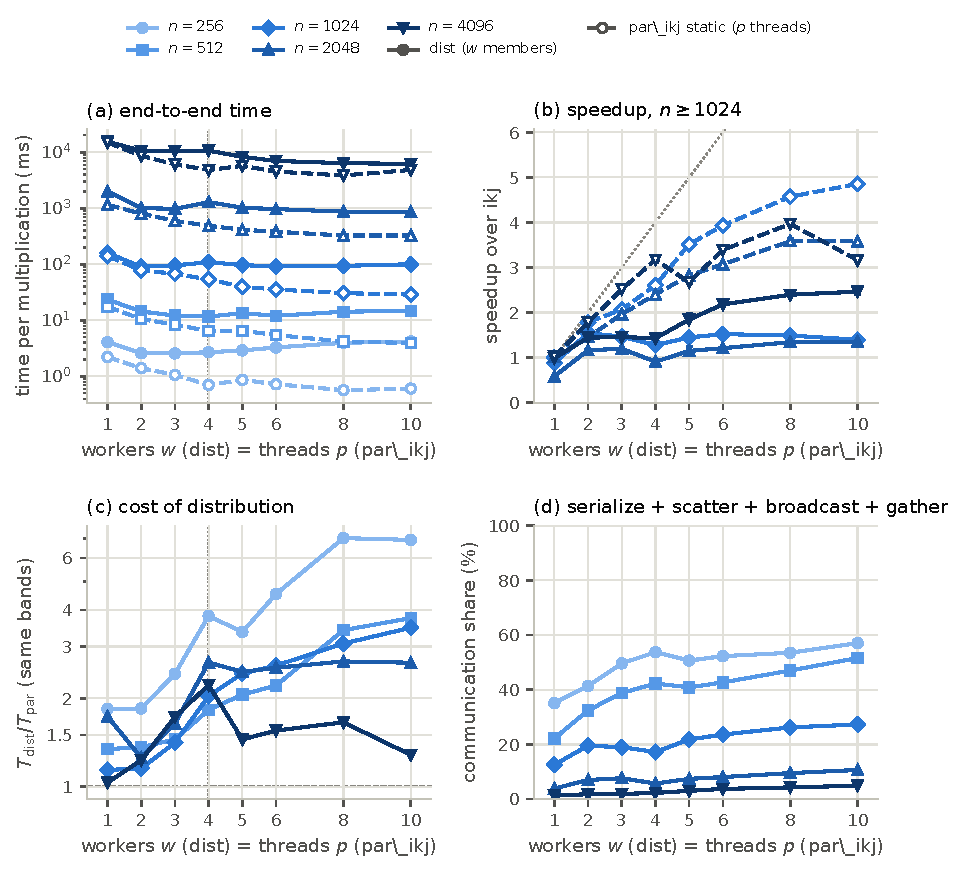
\includegraphics[width=\textwidth]{fig_strong.pdf}
\caption{Strong scaling. (a) End-to-end time (solid: dist with $w$ members;
dashed: par\_ikj static with $p=w$ threads). (b) Speedup over ikj, $n\ge1024$,
with the range of the samples. (c) Time of dist over par\_ikj on the same row
bands. (d) Share of the four communication phases in the time of dist.}
\label{fig:strong}
\end{figure}

Table~\ref{tab:time} and Figure~\ref{fig:strong} give the end-to-end times.
dist is never the fastest method. Its best speedups over ikj are 0.86 at
$n=256$ ($w=3$), 1.49 at $n=512$ ($w=4$), 1.54 at $n=1024$ ($w=2$), 1.35 at
$n=2048$ ($w=10$) and 2.46 at $n=4096$ ($w=10$). For $n\le1024$ its time
stops falling after two to four members and then stays flat or rises; at
$n=2048$ it falls slowly to 862~ms with ten members, and only at $n=4096$ does
it fall clearly with ten members: from 15.5~s with one member to 10.5~s with
two, flat up to four, then down to 6.2~s with ten. par\_ikj on the
same bands reaches 4.85 at $n=1024$ and 3.97 at $n=4096$ ($p=8$). Distributing
the same bands costs between 1.03 and 7.0 times the time of par\_ikj
(Table~\ref{tab:speedup}). Up to $n=2048$ the cost grows with $w$, from 1.1 to
1.9 with one or two members to 2.6 to 6.9 with ten; with ten members it falls
with $n$ from 3.48 at $n=1024$ to 1.28 at $n=4096$. At $n=4096$ it peaks at
2.22 with four members and then falls, because par\_ikj itself slows down there
(five threads are slower than four, and ten slower than eight). With one member the cost is the price of the framework
alone: 1.84 times ikj at $n=256$, 1.14 at $n=1024$ and 1.01 at $n=4096$; at
$n=2048$ it is 1.71, for the reason given in Section~\ref{sec:compute}.

\begin{table}[htbp]
\centering\footnotesize\setlength{\tabcolsep}{3pt}
\caption{Speedup over ikj of dist and of par\_ikj (static, $p=w$), and the
cost of distribution.}
\label{tab:speedup}
\input{\tabledir/tab_speedup.tex}
\end{table}

\subsection{Phases}
\label{sec:phases}

\begin{figure}[htbp]
\centering
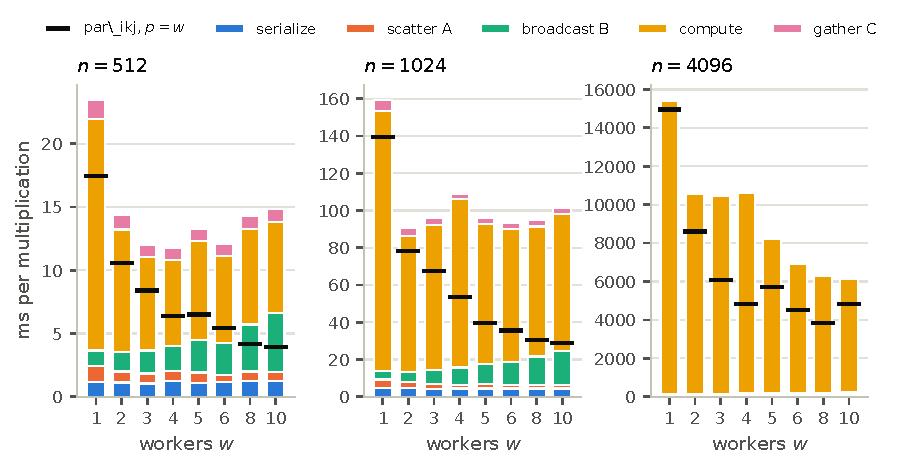
\includegraphics[width=\textwidth]{fig_phases.pdf}
\caption{The five phases of dist, stacked (assemble is included in gather), and
par\_ikj static with $p=w$ (black bars).}
\label{fig:phases}
\end{figure}

Figure~\ref{fig:phases} and Tables~\ref{tab:phases512} and~\ref{tab:phases4096}
split the end-to-end time. At $n=512$ communication (serialize, scatter,
broadcast and gather) is 22\% of the time with one member and 52\% with ten;
the broadcast of $B$ grows from 1.2 to 4.7~ms and is the only phase that grows
with $w$. At $n=4096$ communication is 1.3\% to 4.9\%: scatter (41 down to 26~ms)
and gather (54 to 63~ms) do not grow with $w$, serialize takes 69 to 70~ms up to
$w=3$ and 87 to 98~ms from $w=4$ on for the same bytes, the broadcast grows
from 25 to 129~ms, and the compute phase is the rest. At
$w=10$ the share of communication is 57\%, 52\%, 27\%, 11\% and 4.9\% for
$n=256$ to 4096 (Figure~\ref{fig:strong}d): it halves with each doubling of
$n$ from 1024 on, but falls much more slowly below.

\begin{table}[htbp]
\centering\footnotesize\setlength{\tabcolsep}{4pt}
\caption{Phases of dist at $n=512$ (ms per multiplication).}
\label{tab:phases512}
\input{\tabledir/tab_phases_512.tex}
\end{table}

\begin{table}[htbp]
\centering\footnotesize\setlength{\tabcolsep}{4pt}
\caption{Phases of dist at $n=4096$ (ms per multiplication).}
\label{tab:phases4096}
\input{\tabledir/tab_phases_4096.tex}
\end{table}

\subsection{Compute phase}
\label{sec:compute}

\begin{table}[htbp]
\centering\footnotesize\setlength{\tabcolsep}{2.4pt}
\caption{The compute phase of dist split into its parts, with par\_ikj on the
same bands.}
\label{tab:compute}
\input{\tabledir/tab_compute.tex}
\end{table}

\begin{figure}[htbp]
\centering
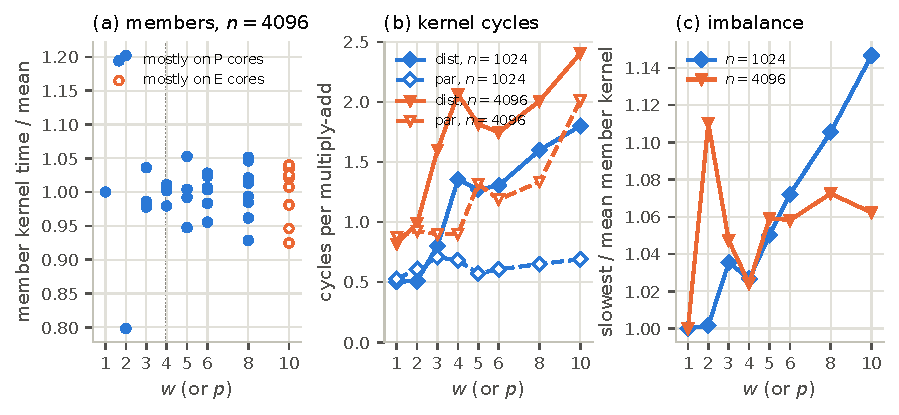
\includegraphics[width=\textwidth]{fig_compute.pdf}
\caption{(a) Kernel time of each member over the mean at $n=4096$, by the core
type the member ran on most. (b) Cycles per multiply-add of the kernels: dist
members (solid) and par\_ikj threads (dashed). (c) Slowest over mean member
kernel.}
\label{fig:compute}
\end{figure}

The compute phase is almost entirely kernel (Table~\ref{tab:compute}): starting
the last task takes at most 0.55~ms after the phase begins, and the last result
reaches the driver at most 0.33~ms after the last task ends. Reading the band
of $A$ and the copy of $B$ out of the member's maps, which deserializes them,
takes 2 to 10~ms at $n=1024$ and 40 to 111~ms at $n=4096$ on the slowest
member.

The kernels of the members are slower than the same bands in par\_ikj. At
$n=1024$ the members need 0.50 cycles per multiply-add with one or two members,
0.80 with three and 1.27 to 1.80 with four to ten, against 0.53 to 0.71 for the
threads of par\_ikj; at $n=4096$, 0.82 to 2.41 against 0.88 to 2.01
(Figure~\ref{fig:compute}b). The members' share of CPU time on P cores is 100\%
up to $w=3$ and falls to 43 to 45\% at $w=10$ (about four members' worth of P
cores), as for threads in Assignment~3. At $n=4096$ a member on E cores is not slower than
one on P cores (Figure~\ref{fig:compute}a: 0.92 to 1.04 of the mean), and the
slowest member is at most 11\% slower than the mean; at $n=1024$ the imbalance
grows with $w$ to 15\% (Figure~\ref{fig:compute}c).

\paragraph{Two speeds of the same kernel.} With one member, the kernel at
$n=2048$ took 1.86 to 2.06~s in four of the five samples and 1.11~s in one. The
instructions were the same in all five (25.4\,G, 2.96 per multiply-add) and the
frequency was the same (4.04~GHz on P cores); only the instructions per cycle
differed: 3.05 to 3.38 against 5.64. The same happened at $n=4096$: 14.8 to
15.4~s with 3.2 to 3.3 instructions per cycle in four samples, and 9.0~s with
5.74 in one, 41\% faster than ikj. ikj in the driver shows the same two levels
at fixed sizes: 5.4 and 5.6 instructions per cycle at $n=2048$ and 2580, 3.1
and 3.25 at $n=3252$ and 4096, again with about 2.9 instructions per
multiply-add. The kernel therefore has two speeds with identical code, and in
the member, which allocates a new band of $C$ and new copies of the inputs for
every task, which one occurs changes from one multiplication to the next. The
slow speed explains why dist with one member costs 1.71 times ikj at $n=2048$.
The cause is not isolated (Section~\ref{sec:discussion}).

\subsection{Data transfer}
\label{sec:transfer}

\begin{table}[htbp]
\centering\footnotesize\setlength{\tabcolsep}{3.5pt}
\caption{Bytes moved per multiplication and effective rates.}
\label{tab:transfer}
\input{\tabledir/tab_transfer.tex}
\end{table}

\begin{figure}[htbp]
\centering
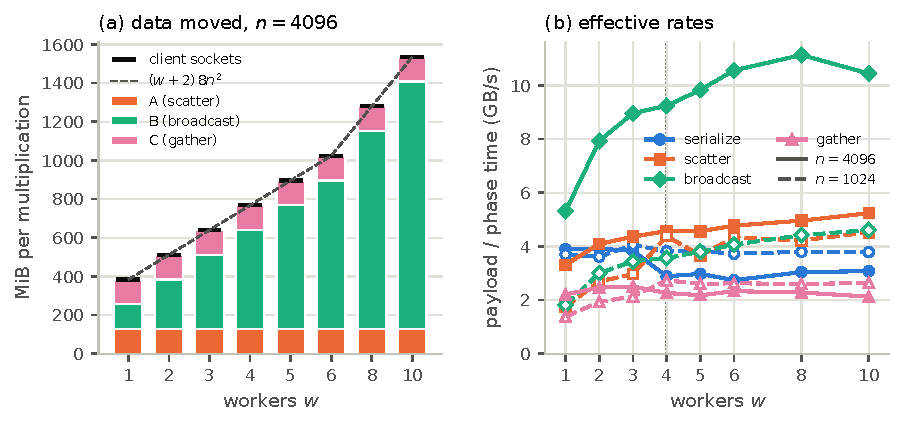
\includegraphics[width=\textwidth]{fig_transfer.pdf}
\caption{(a) Serialized payload per multiplication at $n=4096$ by phase, with
the bytes counted on the client's connections and the model $(w+2)\,8n^2$.
(b) Payload over phase time (solid: $n=4096$; dashed: $n=1024$).}
\label{fig:transfer}
\end{figure}

The serialized payload is the model $(w+2)\,8n^2$ plus the headers of the
bands and rows: 1.0005 times the model at $n=1024$ and 1.00012 at $n=4096$
(Table~\ref{tab:transfer}, Figure~\ref{fig:transfer}a). The bytes on the
client's connections exceed the payload by at most 0.105\% (at $n=256$, with
ten members) and by at most 0.007\% from $n=1024$ on. At $n=4096$ a
multiplication moves 384~MiB with one member and 1\,536~MiB with ten, of which
the copies of $B$ are 128 to 1\,280~MiB. The effective rates (payload over phase
time, on loopback, with serialization, copies and deserialization included) are
at $n=1024$ and 4096, 2.7 to 4.1~GB/s for serialization, 1.8 to 5.2~GB/s for the scatter, 1.4 to
2.7~GB/s for the gather, and 1.8 to 11.1~GB/s for the broadcast, which rises
with $w$, probably because the members receive and store their copies in
parallel. An
empty task takes 78 to 101~$\mu$s to go to a member and back
(Table~\ref{tab:setup}).

\subsection{Setup}
\label{sec:setup-results}

\begin{table}[htbp]
\centering\footnotesize\setlength{\tabcolsep}{3.5pt}
\caption{Setup of a cluster and idle state of the members.}
\label{tab:setup}
\input{\tabledir/tab_setup.tex}
\end{table}

Forming a cluster takes 0.34~s with one member and 9.5 to 11.3~s with two to ten
(Table~\ref{tab:setup}, Figure~\ref{fig:setupmem}a); connecting the client adds
0.29 to 0.40~s. Most of it is each member's start
(\texttt{Hazelcast.newHazelcastInstance}: 7.9 to 10.7~s for $w\ge2$, 0.26~s for
$w=1$, which has no one to wait for). The setup of a given $w$ varies by at
most 2~s over all sizes. With ten members one setup costs as much as about two
multiplications at $n=4096$ and 2\,800 at $n=256$. An idle member uses
5 to 11 thousandths of a core.

\subsection{Memory}
\label{sec:memory}

\begin{table}[htbp]
\centering\footnotesize\setlength{\tabcolsep}{3.5pt}
\caption{Peak memory of the members and of the whole configuration.}
\label{tab:memory}
\input{\tabledir/tab_memory.tex}
\end{table}

\begin{figure}[htbp]
\centering
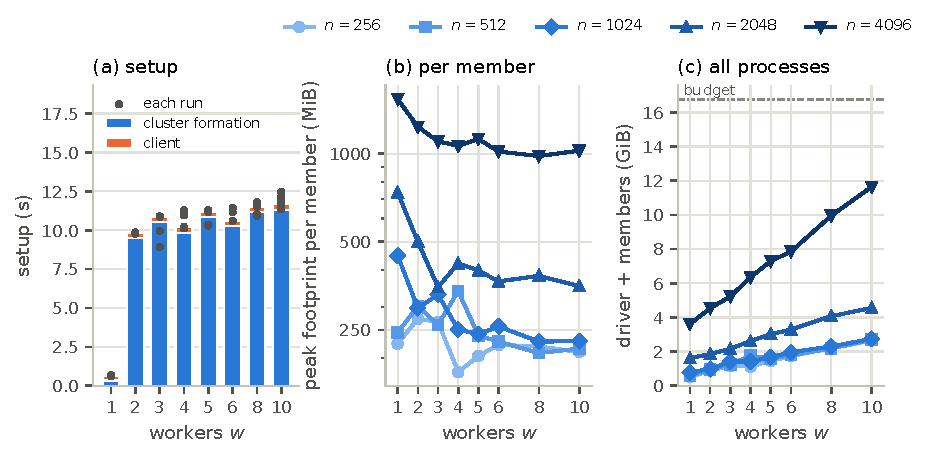
\includegraphics[width=\textwidth]{fig_setup_memory.pdf}
\caption{(a) Setup by number of members (median parts and every run). (b) Peak
memory footprint per member (median). (c) Peak footprint of the driver and all
members, with the declared budget.}
\label{fig:setupmem}
\end{figure}

A member's peak footprint follows its heap limit rather than its data
(Table~\ref{tab:memory}, Figure~\ref{fig:setupmem}b): at $n=4096$ it is 1\,537~MiB
with a 1\,408~MiB limit ($w=1$) and 982 to 1\,237~MiB with 960 to 1\,152~MiB
limits, while the matrices it holds are 154 to 384~MiB; at $n=1024$ it is 228
to 449~MiB against a 576~MiB limit. The garbage collector lets the heap grow towards the limit
before it collects, and the rest is the JVM and Hazelcast. The total grows
linearly with $w$ (Figure~\ref{fig:setupmem}c): at $n=4096$ from 3.6~GiB with
one member to 11.6~GiB with ten, about 0.9~GiB per member, plus 2.1~GiB for the
driver. The largest configuration, $n=8192$ with four members, peaked at
15.8~GiB, within the 16.8~GiB (18~GB) budget.

\subsection{Members and threads on ten cores}
\label{sec:grain}

\begin{table}[htbp]
\centering\footnotesize\setlength{\tabcolsep}{2pt}
\caption{Ten compute threads as $w$ members of $k$ threads.}
\label{tab:grain}
\input{\tabledir/tab_grain.tex}
\end{table}

With the ten cores used as $w$ members of $k$ threads, fewer and larger members
are faster (Table~\ref{tab:grain}, Figure~\ref{fig:grainweak}a). At $n=2048$
the time grows from 395~ms ($1\times10$) to 450, 642 and 862~ms ($2\times5$,
$5\times2$, $10\times1$); at $n=4096$ from 5\,246~ms to 5\,674, 5\,628 and
6\,196~ms ($2\times5$ and $5\times2$ within 1\%). The communication phases change little (72 to 94~ms at $n=2048$, 224
to 304~ms at $n=4096$); the difference is in the compute phase, 314 to 784~ms at
$n=2048$. The members' memory grows from 0.56 to 3.48~GiB at $n=2048$ and from
1.47 to 9.51~GiB at $n=4096$. One member with ten threads is still slower than
par\_ikj with ten threads (395 against 326~ms; 5\,246 against 4\,830~ms).

\begin{figure}[htbp]
\centering
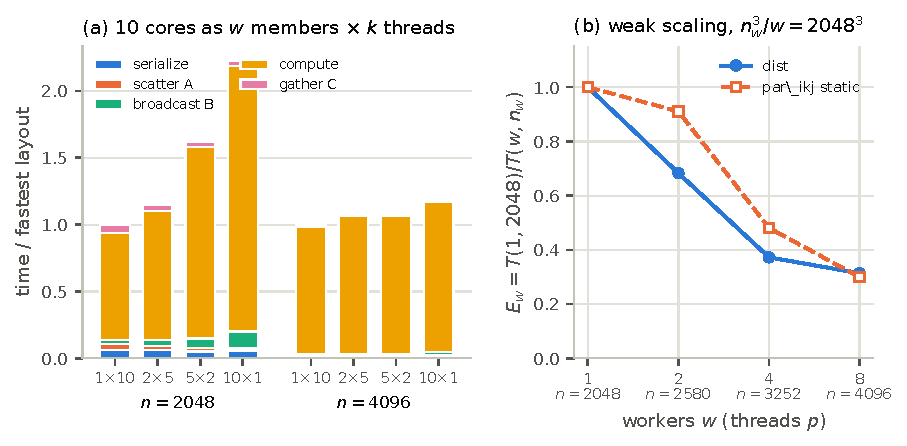
\includegraphics[width=\textwidth]{fig_grain_weak.pdf}
\caption{(a) Ten cores as $w$ members of $k$ threads, phases relative to the
fastest layout of each size. (b) Weak-scaling efficiency with the work per
worker fixed at $2048^3$ multiply-adds.}
\label{fig:grainweak}
\end{figure}

\subsection{Weak scaling}
\label{sec:weak}

\begin{table}[htbp]
\centering\footnotesize\setlength{\tabcolsep}{3.5pt}
\caption{Weak scaling: $n_w^3/w=2048^3$.}
\label{tab:weak}
\input{\tabledir/tab_weak.tex}
\end{table}

With the work per worker fixed (Table~\ref{tab:weak},
Figure~\ref{fig:grainweak}b), the time of dist grows from 2.0~s with one member
to 2.9, 5.4 and 6.4~s with two, four and eight, an efficiency of 0.68, 0.37 and
0.31. par\_ikj falls from 0.91 to 0.48 and 0.30. Communication stays between
2.7\% and 4.3\% of the time of dist although the payload grows from 96 to
1\,280~MiB, so the loss of efficiency is in the compute phase. par\_ikj, with no
communication and one shared $B$, loses almost as much: on one chip a larger
$n$ means more traffic to memory, and beyond four workers the E cores join.
What distribution adds is that dist takes 2.3, 2.2 and 1.7 times as long as
par\_ikj at $w=2$, 4 and 8. The reference
$T(1,2048)$ of dist is itself the slow speed of the kernel
(Section~\ref{sec:compute}); measured against ikj at $n=2048$ (1.17~s) the
efficiency of dist would be 0.40, 0.22 and 0.18.

\subsection{Largest size}
\label{sec:large}

\begin{table}[htbp]
\centering\footnotesize\setlength{\tabcolsep}{3.5pt}
\caption{$n=8192$ (D\_large).}
\label{tab:large}
\input{\tabledir/tab_large.tex}
\end{table}

At $n=8192$ (Table~\ref{tab:large}) ikj took 127.7~s, par\_ikj 61.0~s with four
threads and 61.5~s with ten, and dist with four members 74.6~s (1.22 times
par\_ikj with four threads), with 15.8~GiB of peak memory. The samples of
par\_ikj spread widely: with ten threads 42.5, 61.5 and 70.6~s, while the P
cores' clock fell from 2.01 to 1.52 and 1.51~GHz; with four threads from 2.62 to
1.99 and 1.86~GHz. ikj ran at 3.6~GHz, against 4.04~GHz at every smaller size,
and the members of dist at 1.54 to 1.87~GHz. The machine has no fan: minutes of
work on all cores lower its clock, so these times are those of a hot machine.
The distributed attempt with ten members at this size exceeded the memory
budget in the pilot (Section~\ref{sec:protocol}) and was not repeated.

% ===========================================================================
\section{Discussion}
\label{sec:discussion}

\paragraph{Hypotheses.} Table~\ref{tab:hyp} compares the hypotheses with the
results.

\begin{table}[htbp]
\centering\small
\caption{Hypotheses (Section~1) against the results.}
\label{tab:hyp}
\begin{tabular}{>{\raggedright}p{0.6cm}>{\raggedright}p{2.2cm}>{\raggedright\arraybackslash}p{11.6cm}}
\toprule
& Verdict & Evidence \\
\midrule
H1 & supported & One checksum per size over all methods and configurations; 189 bitwise checks before the session (Section~\ref{sec:placement}). \\
H2 & supported & Cluster plus client connection: 0.6~s with one member, 9.8 to 11.8~s with two to ten, varying by at most 2~s over sizes (Section~\ref{sec:setup-results}). \\
H3 & mostly supported & Payload within 0.05\% of $(w+2)\,8n^2$; socket overhead below 0.11\% (below 0.01\% for $n\ge1024$). Distribution time grows with $w$ through the broadcast only, and less than linearly, because the broadcast's rate rises with $w$ (5.3 to 11~GB/s at $n=4096$) (Section~\ref{sec:transfer}). \\
H4 & partly supported & dist is slower than ikj at $n=256$ (best 0.86) but not at $n=512$ (up to 1.49). The communication share halves with each doubling of $n$ from 1024 on, but between 256 and 512 it barely moves (57\% to 52\% at $w=10$): per-message costs dominate there, not bytes (Section~\ref{sec:phases}). \\
H5 & supported for $w\ge3$ & The members need 1.27 to 1.80 cycles per multiply-add at $n=1024$ with four to ten members, against 0.57 to 0.69 for par\_ikj; at $n=1024$ with two members dist computes slightly faster than par\_ikj (Section~\ref{sec:compute}). \\
H6 & not supported & At $n=4096$ members on E cores are not slower than members on P cores and the imbalance is at most 11\%; dist gains from $w=4$ to 5 at $n=1024$, 2048 and 4096 (Section~\ref{sec:compute}). \\
H7 & supported, other cause & $1\times10$ fastest and $10\times1$ slowest at both sizes, but communication changes little; the difference is the compute phase (Section~\ref{sec:grain}). \\
H8 & partly supported & Total memory grows linearly with $w$ (0.9~GiB per member at $n=4096$), but a member's footprint follows its heap limit, not its data (Section~\ref{sec:memory}). \\
H9 & supported, other cause & Efficiency falls to 0.31 at $w=8$, but communication stays below 5\%; the loss is in the compute phase, and par\_ikj loses as much (0.30), so most of it is the shared machine, not distribution (Section~\ref{sec:weak}). \\
\bottomrule
\end{tabular}
\end{table}

\paragraph{Where the time goes.} The results separate two costs of
distribution. The first is communication: serializing, sending, receiving and
deserializing $(w+2)\,n^2$ doubles plus a few round trips per multiplication.
Its bytes are exactly predictable, and on loopback it moves 2 to 11~GB/s, so it
dominates only at $n\le512$, where a multiplication is a few milliseconds. The
second, larger from $n=1024$ on, is that the members compute more slowly than
threads on the same bands. Each member owns a private copy of $B$: where
par\_ikj's threads read one $B$ through the shared caches, $w$ members read $w$
copies, so the traffic between the caches and memory grows with $w$. The cycles
per multiply-add grow with the number of members accordingly (1.27 to 1.80 at
$n=1024$, where one 8~MiB copy fits in the 16~MiB L2 cache of the P cores and
four do not), while the instructions do not change. The same effect explains
why fewer, larger members are faster on the same ten cores (H7) and why dist
stays 1.7 to 2.3 times slower than par\_ikj in weak scaling with almost no
communication; the fall of efficiency itself (H9) is shared with par\_ikj and
comes from running more work on one chip. The core
type matters less than predicted (H6): at $n=4096$ the members are limited by
memory, as par\_ikj was in Assignment~3, so a member on an E core keeps up with
one on a P core.

\paragraph{Fixed costs.} Starting a cluster costs about 10~s, most of it
Hazelcast's wait for further members before it forms a cluster. It is paid once
per cluster, so a cluster kept alive across many multiplications amortises it,
and a cluster started for one multiplication does not: 10~s is more than the
whole dist run at $n=4096$ with ten members. Round trips of about 0.1~ms and
the client's per-operation work set a floor of about 2.5~ms per multiplication
at $n=256$, which is why dist never beats ikj there.

\paragraph{Two speeds of the kernel.} The same ikj code runs at about 5.5 or
about 3.2 instructions per cycle, with the same instructions and clock
(Section~\ref{sec:compute}). Assignment~1 left open why Java was slow at some
power-of-two sizes, and Assignment~2 why ikj needed more time per multiply-add
at $n=3072$ than at 4096. The new evidence is that the slow speed is not tied
to $n$: one member changed speed between consecutive multiplications of the
same size, as its arrays were allocated again. This points to the relative
addresses of the rows of $B$ and $C$ (for instance conflicts in the cache sets
or false dependences between stores to $C$ and loads from $B$ at nearby
addresses modulo the page size) rather than to the size. That is a hypothesis;
it was not tested here, for example by padding the rows or controlling their
alignment.

\paragraph{Limitations.}
\begin{itemize}
  \item Local execution. All processes ran on one machine over loopback, with
  the instructor's permission requested for the only machine available. No
  physical network was measured: the transfer times include serialization and
  copies through the kernel, not network latency or bandwidth. The members
  compete for one machine's cores, caches and memory bandwidth, which on
  separate machines they would not; the slower compute of the members is
  partly a property of sharing one chip, and the cluster's memory is the memory
  of one machine.
  \item Heterogeneous cores without affinity. macOS places threads and processes
  on P and E cores; the counters measure where they ran but cannot control it.
  \item Thermal state. The machine has no fan; at $n=8192$ the clock fell by up
  to 25\% within three samples, and the times there describe a hot machine.
  \item Kernel speed. The two speeds of the kernel add variance between
  configurations that is not caused by distribution; the dist results with one
  member at $n=2048$ and 4096 and the weak-scaling reference are the most
  affected.
  \item Design. The 1D decomposition replicates $B$; a 2D decomposition such as
  SUMMA~\cite{vandegeijn1997} would send less and store less per member. The
  maps have no backups, so a member failure loses data. Each configuration was
  measured in one session, with five samples (three at $n=8192$).
\end{itemize}

% ===========================================================================
\section{Conclusions}
\label{sec:conclusions}

On one machine, a row-band multiplication on a Hazelcast cluster is correct
(bitwise identical to the sequential kernel for every configuration) and
predictable in what it moves, $(w+2)\,8n^2$ bytes within 0.05\%, but it is
never faster than the shared-memory parallel version on the same cores. Its
best speedup over ikj is 1.4 to 1.5 for $n=512$ to 2048 and 2.5 at $n=4096$,
against 3.6 to 4.9 for par\_ikj; distributing the same bands costs 1.03 to 7 times
par\_ikj's time. Communication dominates only for small matrices; from
$n=1024$ on the main cost is that $w$ processes with $w$ private copies of $B$
compute more slowly than threads sharing one, which also makes fewer and
larger members faster and keeps dist 1.7 to 2.3 times slower than the threads
in weak scaling. Starting a cluster takes about 10~s, which only a long-lived cluster
amortises. These are the costs of the framework and of separate processes on a
shared chip; the cost of a real network, and the benefit of the memory and
memory bandwidth of more machines, remain to be measured on a real cluster.

% ===========================================================================
\section{References and materials}
\label{sec:materials}

\paragraph{Reproducibility materials.} All code, data and scripts are in the
directory \texttt{assignment4/} of the GitHub repository below, at the tag
\texttt{assignment4-v1.1}:
\begin{center}\repourl\end{center}
Its README gives the exact build and run commands and the software versions.
The materials are:
\begin{itemize}
  \item \texttt{src/}: the Java methods, the Hazelcast code (configuration,
  serializable classes, tasks, driver side, member process), the benchmark
  driver and the JUnit tests; \texttt{pom.xml}: the Maven build.
  \item \texttt{config/bench.json}: the declared protocol, read by every script;
  it includes the Hazelcast settings, which are applied by
  \texttt{HazelcastSetup.java}.
  \item \texttt{scripts/}: input generation (\texttt{gen\_inputs.py}),
  correctness verification on real multi-process clusters (\texttt{verify.py}),
  the member launcher (\texttt{cluster.py}), the benchmark harness
  (\texttt{run\_benchmarks.py}) and the environment snapshot.
  \item \texttt{data/checksums.sha256}: the digests of the inputs, which are
  regenerated in a few seconds instead of being stored.
  \item \texttt{results/correctness.csv}: the outcome of the correctness checks.
  \item \texttt{results/raw/\session/}: every raw sample, warm-ups included
  (\texttt{samples.csv}), every member's task timers and counters
  (\texttt{member\_samples.csv}), one row per configuration and one per member
  process (\texttt{runs.csv}, \texttt{members.csv}), the environment snapshot
  (\texttt{env.txt}) and the protocol used (\texttt{config.json}).
  \item \texttt{analysis/analyze.py}: the script that produces every table and
  figure in this report from the raw data.
\end{itemize}

\paragraph{Reuse of Assignments 1 to 3.} The kernels (basic, ikj, par\_ikj),
the dense file format, the process counters, the input generator and its files,
the correctness tolerance, and the structure of the benchmark driver, the
harness, the verification script, the environment snapshot and the analysis
script come from Assignment~3 at the tag \texttt{assignment3-v1.0} (which took
basic from Assignments~1 and~2). Each reused file names its origin.

\paragraph{Use of generative AI.} Claude Code (Anthropic, model Claude Opus~5.5)
was used as a programming and writing assistant. It helped plan the study,
read Hazelcast's source code to find the interfaces for the placement and the
byte counters, draft and debug the Java code, tests, scripts and analysis,
diagnose the memory limit found in the pilot and the sleep and background-load
problems that led to discarding two sessions, analyse the counters behind the
two speeds of the kernel, and draft and revise the text of this report. All measurements were produced by running the code on the author's
machine, and every result in Section~\ref{sec:results} is computed from the
committed data by the scripts in the repository. Each cited source was checked
against the original publication or documentation. The author reviewed the
code and the text and is responsible for the work and its conclusions.

\renewcommand{\refname}{References}
\begin{thebibliography}{99}\raggedright
\small

\bibitem{a3report}
M.~Prosperi Reynoso, ``Assignment 3: Parallel matrix multiplication in Java,''
BIG DATA individual assignment report, ULPGC, Nov. 2026. [Online]. Available:
\url{https://github.com/Xami650/Individual-Assignments-Big-Data-ULPGC/tree/assignment3-v1.0/assignment3}

\bibitem{grama2003}
A.~Grama, A.~Gupta, G.~Karypis, and V.~Kumar, \emph{Introduction to Parallel
Computing}, 2nd~ed. Harlow, U.K.: Addison-Wesley, 2003, ch.~8.

\bibitem{cannon1969}
L.~E. Cannon, ``A cellular computer to implement the Kalman filter
algorithm,'' Ph.D. dissertation, Montana State Univ., Bozeman, MT, USA, 1969.

\bibitem{vandegeijn1997}
R.~A. van~de~Geijn and J.~Watts, ``SUMMA: Scalable universal matrix
multiplication algorithm,'' \emph{Concurrency: Practice and Experience},
vol.~9, no.~4, pp.~255--274, 1997.

\bibitem{hockney1994}
R.~W. Hockney, ``The communication challenge for MPP: Intel Paragon and Meiko
CS-2,'' \emph{Parallel Computing}, vol.~20, no.~3, pp.~389--398, 1994,
doi: 10.1016/S0167-8191(06)80021-9.

\bibitem{amdahl1967}
G.~M. Amdahl, ``Validity of the single processor approach to achieving large
scale computing capabilities,'' in \emph{Proc. AFIPS Spring Joint Computer
Conf.}, vol.~30, Atlantic City, NJ, USA, Apr. 1967, pp.~483--485.

\bibitem{gustafson1988}
J.~L. Gustafson, ``Reevaluating Amdahl's law,'' \emph{Commun. ACM}, vol.~31,
no.~5, pp.~532--533, May 1988, doi: 10.1145/42411.42415.

\bibitem{hzrelease}
Hazelcast, Inc., ``Community Edition release notes,'' \emph{Hazelcast Platform
5.7 Documentation}. Accessed: Nov.~18, 2026. [Online]. Available:
\url{https://docs.hazelcast.com/hazelcast/5.7/release-notes/community}

\bibitem{hzaffinity}
Hazelcast, Inc., ``Data affinity,'' \emph{Hazelcast Platform 5.7
Documentation}. Accessed: Nov.~18, 2026. [Online]. Available:
\url{https://docs.hazelcast.com/hazelcast/5.7/cluster-performance/data-affinity}

\bibitem{hzexecutor}
Hazelcast, Inc., ``Java executor service,'' \emph{Hazelcast Platform 5.7
Documentation}. Accessed: Nov.~18, 2026. [Online]. Available:
\url{https://docs.hazelcast.com/hazelcast/5.7/computing/executor-service}

\bibitem{hzclient}
Hazelcast, Inc., ``Java client,'' \emph{Hazelcast Platform 5.7 Documentation}.
Accessed: Nov.~18, 2026. [Online]. Available:
\url{https://docs.hazelcast.com/hazelcast/5.7/clients/java}

\bibitem{hzserialization}
Hazelcast, Inc., ``Serializing objects and classes,'' \emph{Hazelcast Platform
5.7 Documentation}. Accessed: Nov.~18, 2026. [Online]. Available:
\url{https://docs.hazelcast.com/hazelcast/5.7/serialization/serialization}

\bibitem{hzreplicated}
Hazelcast, Inc., ``Replicated map,'' \emph{Hazelcast Platform 5.7
Documentation}. Accessed: Nov.~18, 2026. [Online]. Available:
\url{https://docs.hazelcast.com/hazelcast/5.7/data-structures/replicated-map}

\bibitem{hzproperties}
Hazelcast, Inc., ``System properties,'' \emph{Hazelcast Platform 5.7
Documentation}. Accessed: Nov.~18, 2026. [Online]. Available:
\url{https://docs.hazelcast.com/hazelcast/5.7/system-properties}

\bibitem{hzbackups}
Hazelcast, Inc., ``Making your map data safe,'' \emph{Hazelcast Platform 5.6
Documentation}. Accessed: Nov.~18, 2026. [Online]. Available:
\url{https://docs.hazelcast.com/hazelcast/5.6/data-structures/backing-up-maps}

\bibitem{georges2007}
A.~Georges, D.~Buytaert, and L.~Eeckhout, ``Statistically rigorous Java
performance evaluation,'' in \emph{Proc. 22nd Annu. ACM SIGPLAN Conf.
Object-Oriented Programming Systems, Languages and Applications (OOPSLA)},
2007, pp.~57--76, doi: 10.1145/1297027.1297033.

\bibitem{higham2002}
N.~J. Higham, \emph{Accuracy and Stability of Numerical Algorithms}, 2nd~ed.
Philadelphia, PA, USA: SIAM, 2002.

\bibitem{macsdk}
Apple Inc., \texttt{<sys/resource.h>} (\texttt{struct rusage\_info\_v6}) and
\texttt{<libproc.h>} (\texttt{proc\_pid\_rusage}, \texttt{proc\_pidinfo}), macOS
SDK of the Command Line Tools for Xcode, header files.

\bibitem{applem4}
Apple Inc., ``MacBook Air (15-inch, M4, 2025) -- Tech Specs,'' Apple Support.
Accessed: Nov.~4, 2026. [Online]. Available:
\url{https://support.apple.com/en-us/122210}

\bibitem{harris2020}
C.~R. Harris \emph{et al.}, ``Array programming with NumPy,'' \emph{Nature},
vol.~585, no.~7825, pp.~357--362, Sep. 2020, doi: 10.1038/s41586-020-2649-2.

\end{thebibliography}

\end{document}
